\section{Introduction}
\label{sec:introduction}

In the context of vehicle-to-vehicle (V2V) or vehicle-to-infrastructure (V2I) communication, communication often involves the exchange of spatial information to anchor data to a specific location, be it a point, a line or an area.

An example for system that broadcasts such information is the Radio Data System Traffic Message Channel , or short RDS-TMC \cite{tmc} standard (maintained by the Traveller Information Service Association \cite{TISA}) that is used to propagate information about the traffic situation such as the length traffic jams or the location of accidents and weather conditions. RDS-TMC makes use of a lookup table in which events and a locations are assigned to unique identifiers. In order to work correctly the receiver has to use the same version of the lookup table as the broadcaster. It is obvious that while the system works very efficient it can not scale to describe all possible roads or locations. 

Location referencing systems such as Open LR\tm try to solve the problem of exchanging information about locations in a more dynamic approach. The rely on communicating real world properties such as the geo-coded location using GPS\footnote{Global Positioning System} to describe a location. The problem is that two different parties can have different understandings of where a location might be, because they have access to different maps.

\section{Open LR\tm}
\label{sec:open_lr}

Open LR\tm tries to solve the problem of exchanging location properties unambiguously with a second party regardless of map differences. 

% TODO Was wird bei Open LR als Location verstanden

The main idea of Open LR\tm is to make use of the shortest path algorithm. It tries to reduce the number of edges and nodes by computing a series of shortest paths that covers the location. Each of these shortest paths can be defined only by their start and end node, so that only a short series of nodes have to be used to encode a location. The decoding party then matches these point to its own map and runs a series of shortest path algorithms to determine the location being referenced.

To do so Open LR\tm relies on a few features or rather qualities of a map. The system needs access to the geo-coded locations of each node (using WGS84 ???). Each edge should know about the real world geometry, such as the length in meter. Also the the standard explicitly asks to support two attributes for each road, the \emph{form of way }and a \emph{functional road class}.

The form of way describes the physical appearance that an edge takes in real life, a motor-way, a multiple/single carriage-way or a traffic square. The functional road class is a more abstract classification based on the importance of a road. Possible values range from 0, as a main road, to 7, as a road of less or unknown importance. These attributes help to find the right candidate nodes and edges when trying to decode the location reference.

\emph{Both maps, the encoder map, and the decoder map should meet certain \"navigable standards\" in terms accuracy and content.  describe a a graph describing the street network.}. This papers explores and questions the idea of what \"navigable standard\" standards means.

%TODO das geht besser

A street network can be described as a graph, the connection of various nodes, of which the geographical location is known. Ideally these nodes represent crossroads in real life.

A location can be defined by a series of nodes. As the protocol will be heavily used by mobile systems, ideas to efficiently compress the information is needed. In order to reduce the number of points that have to be communicated Open LR\tm employs a shortest path algorithm. If the way the driver has chosen happens to be the shortest path between the two outer most nodes describing his way, Open LR\tm binary encodes the location as a location reference in a compact way and pushes it to the communication interface. If the shortest path differs from the way the driver tries to communicate, Open LR takes the node at which the way differs as a supporting node and starts the shortest algorithm between this node and the end node until the location reference is found.

In short Open LR\tm builds a location reference by calculating the shortest path between two nodes, saving the the differences between the real location and the location reference. The position of the  starting node is encoded absolutely, while the positions of all following nodes are saved relative to the first, thus saving space. Furthermore Open LR saves information such as the form of way, the functional road class and the bearing of the road to help the decoding party find the correct node.

The decoding party takes the information given and tries to map the encoded nodes to its network, having hopefully access to the same kind of information, but realistically relying on different maps and data sets. Often the data provided by the underlying systems differs from the encoded data. The decoding algorithm has to implement heuristic methods to match the geo-coded node to one of the nodes stored in system of the decoding party. While this can be done with simple geometric calculations, the extra information, such as the form of way, the functional road class, and also the bearing might help the system find the correct candidate, if there are multiple choices.

\section{Example}
\label{sec:open-lr-example}

The example from the white paper shows us this excerpt from a map. Of course it only shows the abstract information that is available to the system.

\begin{figure}
  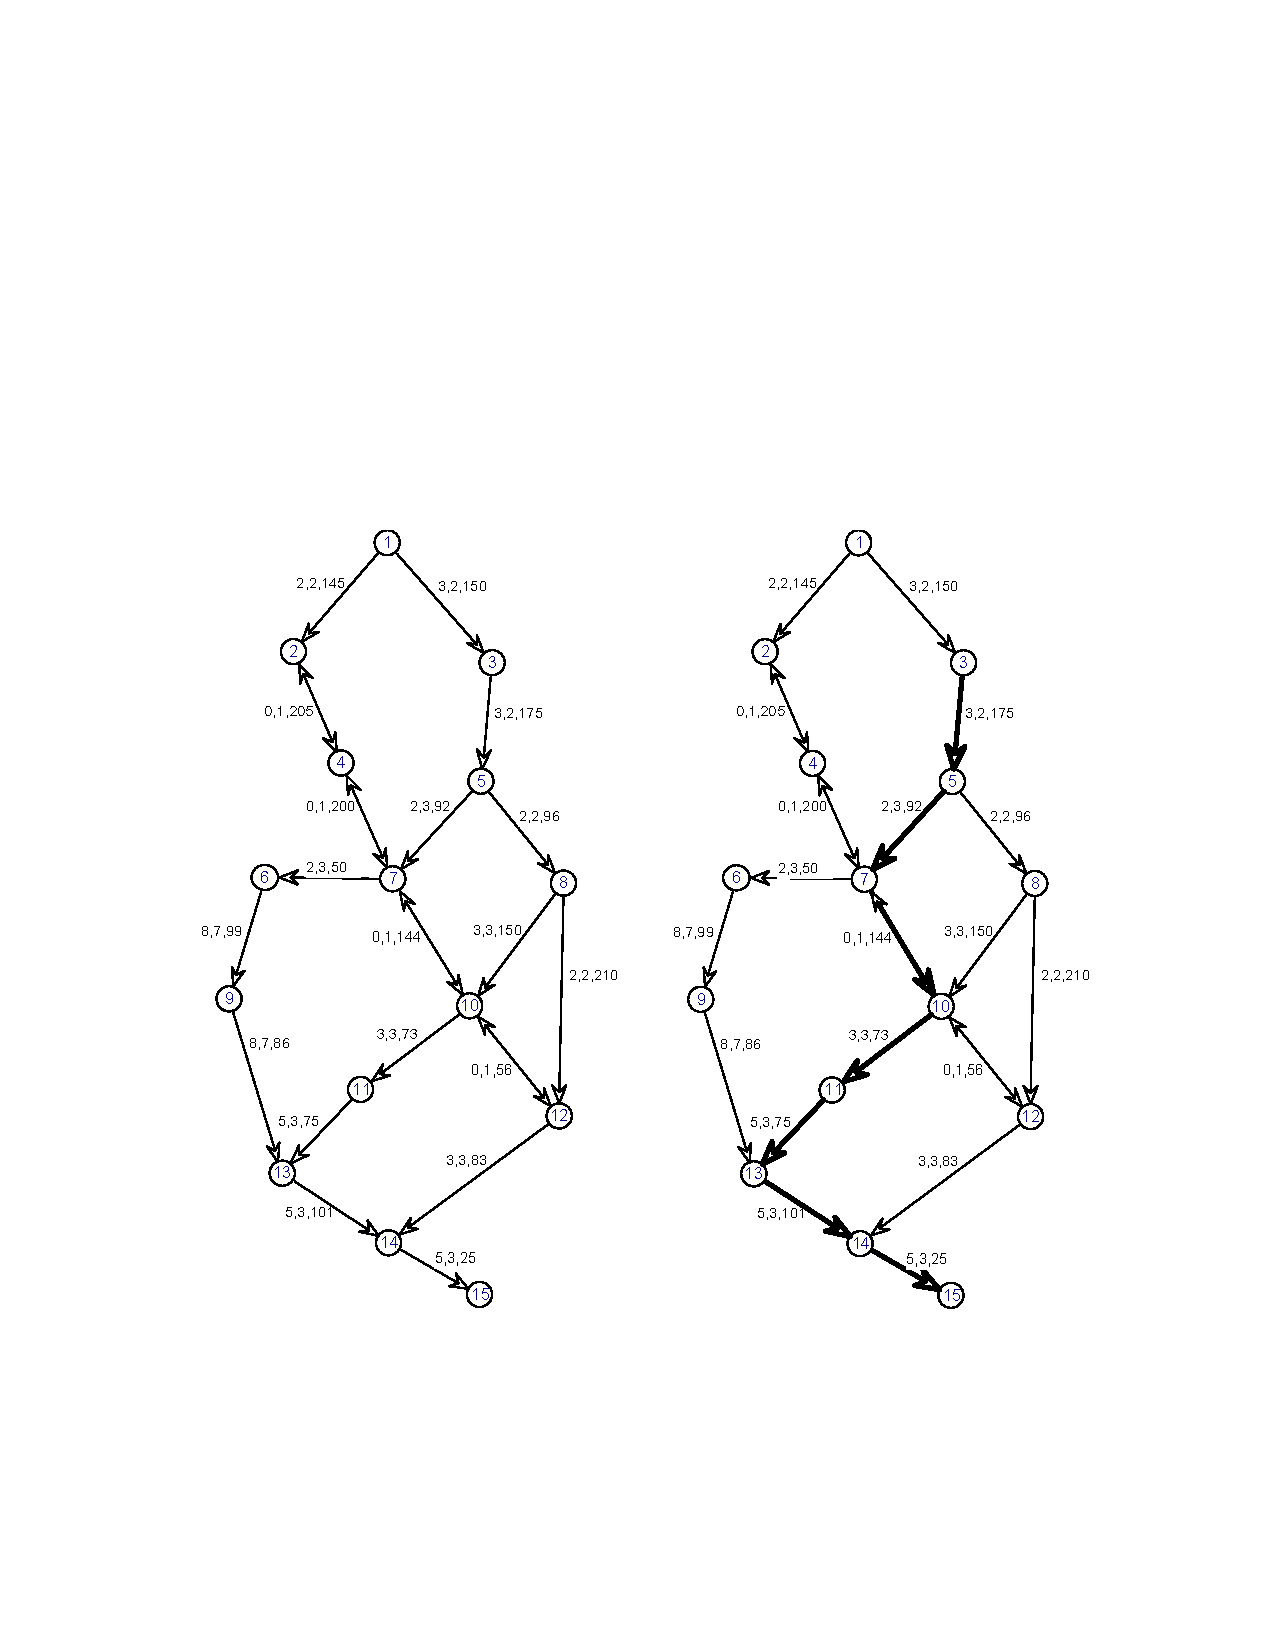
\includegraphics{openlr-encoding-1.pdf}%
  \caption{\emph{Open LR - choosing a location to encode}}%
  \label{fig:openlr-encoding-1}%
\end{figure}

In the example the driver wants to encode the location along the nodes 3, 5, 7, 10, 11, 13, 14, 15. The values tagged to to edges of the between the nodes represent the the functional road class, the form of way and the distance to the next point in meters.

\begin{figure}
  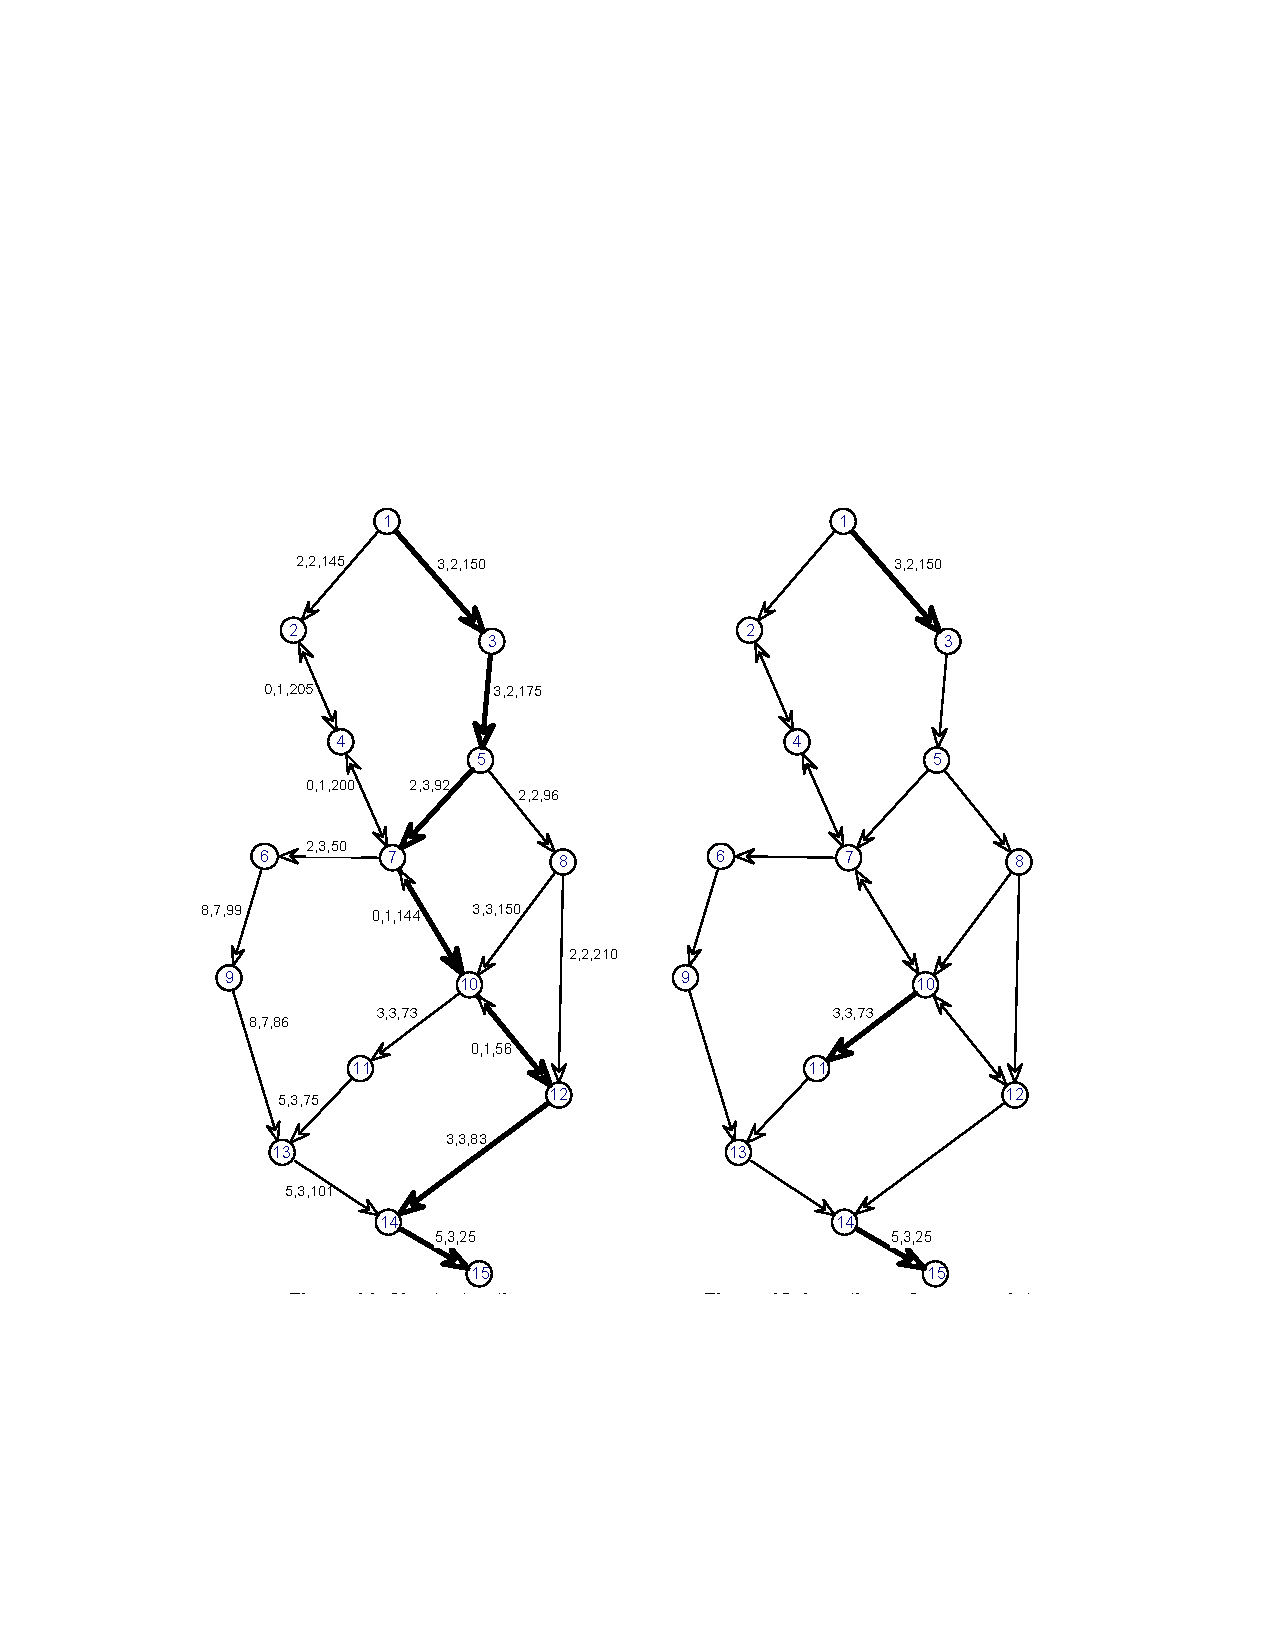
\includegraphics{openlr-encoding-2.pdf}%
  \caption{\emph{Open LR - encoding location reference nodes}}%
  \label{fig:openlr-encoding-2}%
\end{figure}

In order to encode the location the system first has to make sure that the location about to be encoded is a valid one. It checks whether the location is connected, which it is in this case and if the system has data for the functional road class attached to all streets, which it also has. A real system might also want to check if the location described includes turn restrictions. According to the use case this behavior might desirable or not, in this example it is not needed.

Having validated the location, the system now has to build a location reference. According to the ruleset the start and end point of a valid location reference point only allows for one incoming and one outgoing line. This should meet the restriction that in the real world nodes should represent junctions. While the end point, node 15, conforms the rule, the start node, node 3, does not. To conform, the start node has to be extended to node 1. To communicate the correct starting point of the location and offset is set, in this case, to 150 meter.

The encoder then proceeds calculating the shortest path between node 3 (node 1 was included in the extension phase and can be ignored) and 15. If the path has been calculated, it compares the result to the location that should be encoded. If the encoder finds deviation, it will restart the process again from the deviating edge. The nodes will be added to the location reference as supporting nodes.

In this case the encoder is very efficient and only has to store one deviation, thus one supporting node in addition to the start and end node. The nodes in question are:

\begin{table}
  \centering
  \begin{tabular}{ l l l l l l }
    Node ID  & LRP index & Longitude & Latitude & Relative longitude & Relative latitude \\
    1 & 16.12683° & 49.60851° & --- & --- \\
    10 & 2 & 6.12838° & 49.60398° & 155 & -453 \\
    15 & 3 & 6.12817° & 49.60305° & -21 & -93 \\
  \end{tabular}
  \caption{Encoded nodes}
  \label{tab:encoded_nodes}
\end{table}

The relevant metadata is:

\begin{table}
  \centering
  \begin{tabular}{ l l l l l l }
    LRP index & FRC & FOW & BEAR & LFRCNP & DNP \\
    1 & FRC3 & MULTIPLE CARRIAGEWAY & 135\degree & FRC3 & 561 \\
    2 & FRC3 & SINGLE CARRIAGEWAY & 227\degree & FRC5 & 274 \\
    3 & FRC5 & SINGLE CARRIAGEWAY & 290\degree & --- &  --- \\
  \end{tabular}
  \caption{Relevant data}
  \label{tab:relevant_data}
\end{table}

In addition to that the system also takes into account the offset of 150 m to get to the real starting point.

Once transmitted to the decoding party, the decoding unpacks the binary data and starts to decode the location reference by finding the candidate nodes for the location reference points.

\begin{figure}
  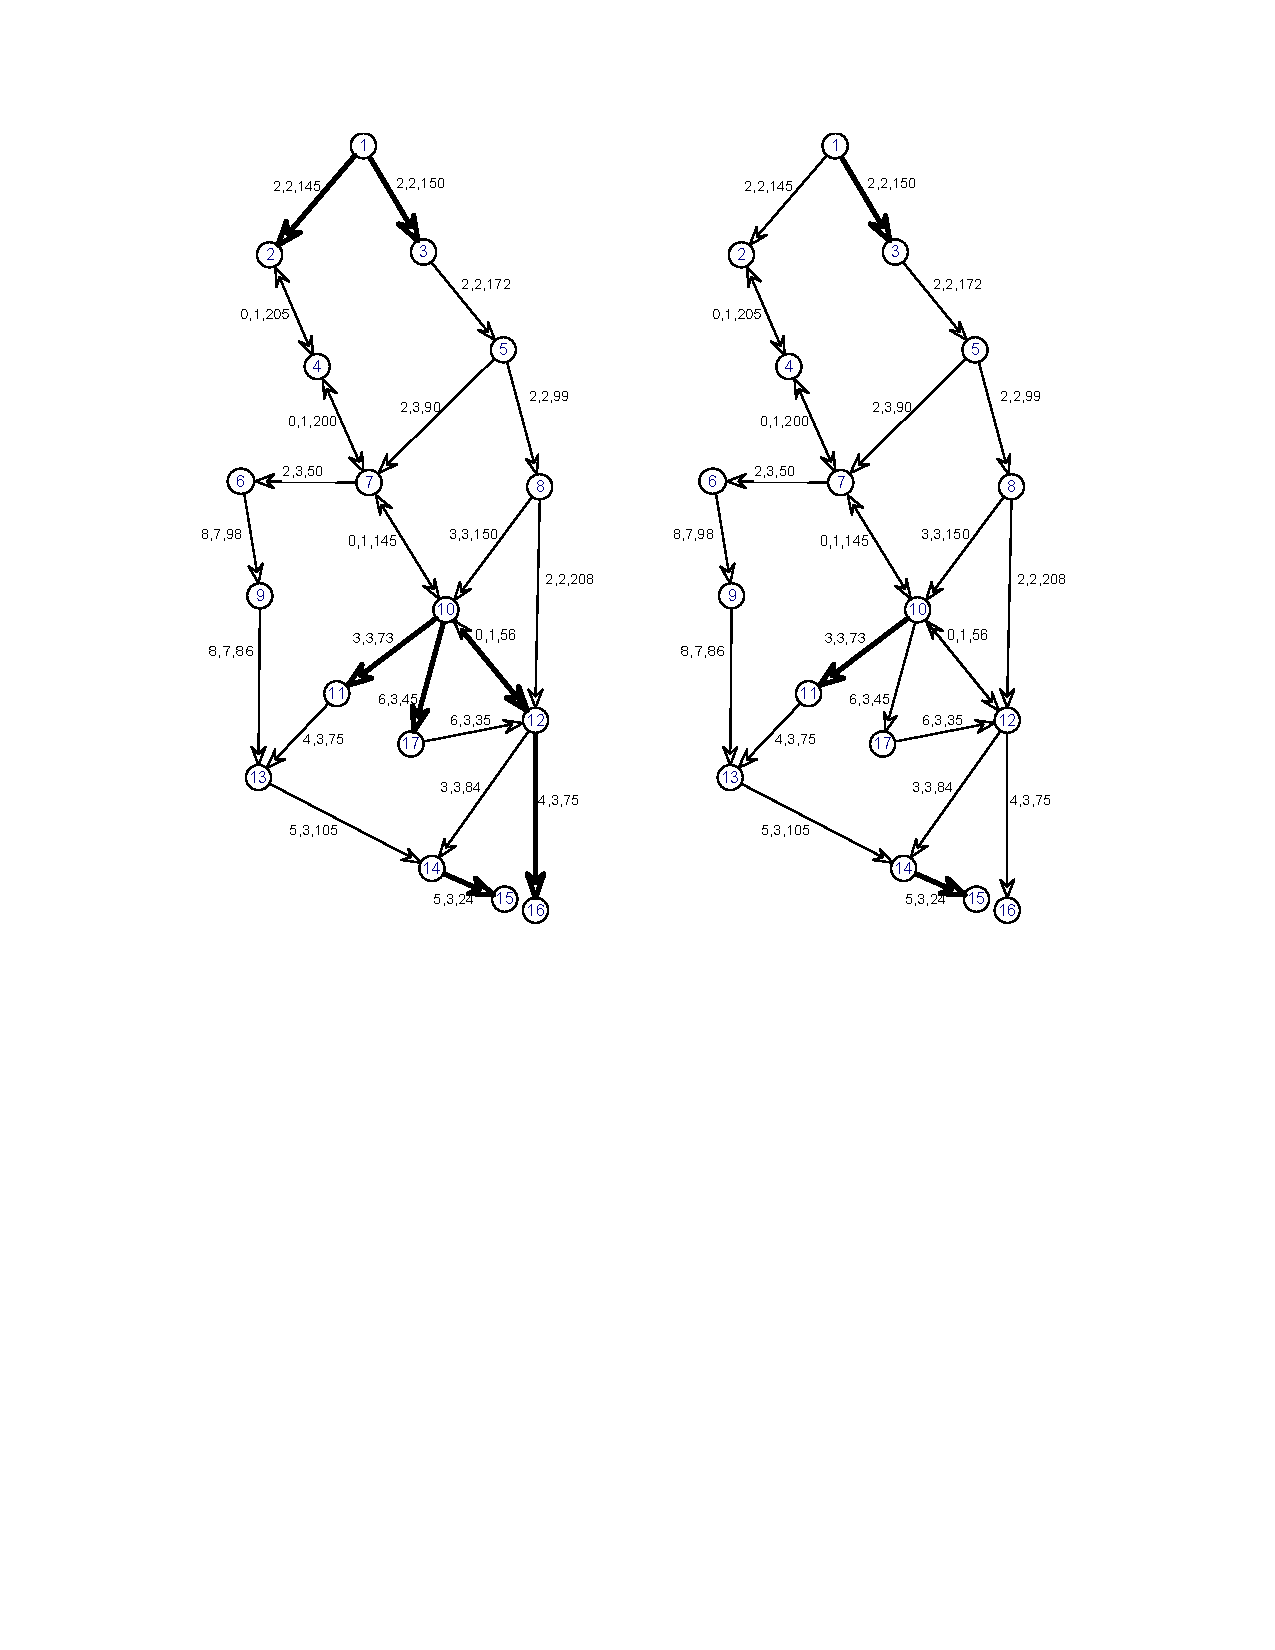
\includegraphics{fig/openlr-decoding-1.pdf}%
  \caption{\emph{Open LR - choosing the candidates for decoding}}%
  \label{fig:openlr-decoding-1}%
\end{figure}

How exactly the decoding party should select is not exactly specified, but it is recommended to take all data into account that is available. That means not only to resolve the best candidate by geometric means, but also taking other criteria such as the functional road class, the form of way and the bearing into account.

If the candidates have been chosen and accordingly matched to nodes of the decoding party, the decoding party in turn calculates the shortest path between sequential pairs of the transmitted location reference points.

The decoder should fail if it does not find matching nodes or lines according to his employed metrics.

\section{Problem} 
\label{sec:openlr-problem}

The Open LR protocol and format works well if the underlying data sets of both, the encoding and decoding party are of high quality. The white paper states that the maps have to be \"navigable maps\". 

The concept of Open LR relies heavily on the shortest path algorithm. This makes it a prerequisite for the map to be of a certain quality, implying an up to date and more or less complete map, because missing or additional links could lead to failures of the decoder. 

The algorithm has a rather crucial problem. It might communicate the wrong location if the idea of the shortest path between two nodes differ on the decoder. While this case should be rather seldom, especially in well mapped urban areas, it could happen in not so densely populated or rarely visited areas.

Consider the same example as above, but now the decoding map has one additional link between node 3 and node 5. In reality this case could mean that a bypass has been built and that the map data of the encoding party has not been updated no include the change. In more abstract terms this problem describes just the case that two different links are candidates for the decoder leaving it up to the implementation to choose the correct or incorrect one or even fail completely. 

\begin{figure}
  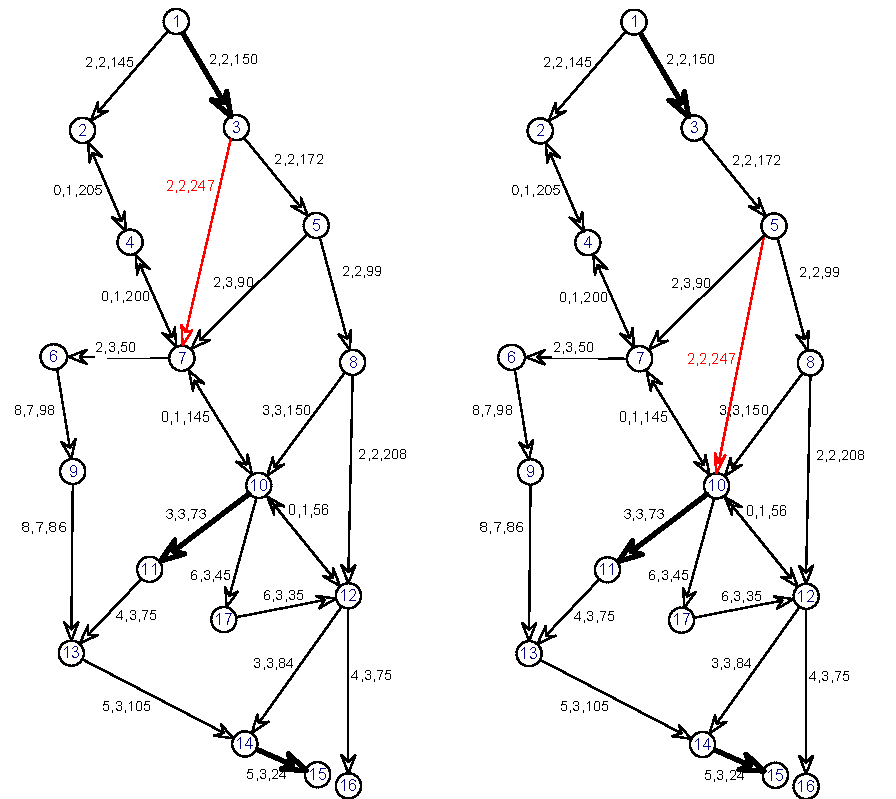
\includegraphics{fig/openlr-decoding-2.pdf}%
  \caption{\emph{Open LR - decoding with alternate routes}}%
  \label{fig:openlr-decoding-2}%
\end{figure}

The decoder does not have a problem choosing the right candidate node in terms of the geo-coded location, for the sake of the argument they are the same. The implementation should not be thrown off by the fact that there is another link when choosing the candidate node.

It might have problems though when calculating the shortest path though. The new link has the same functional road class and the same form of way. There are two informations that (might) deviate though, the bearing and the length.

When calculating the path between node 3 and node 10 there are now three possible routes (please note the direction of the roads). 

\begin{itemize}
	\item Through node 1, 3, 5, 7 to 10 resulting in a length of 150 + 172 + 90 + 145 = 557  
	\item Through node 1, 3, 5, 8 to 10 resulting in a length of 150 + 172 + 99 + 150 = 571
	\item Through node 1, 3, 7, 10 resulting in a length of 150 + 247 + 145 = 542  
\end{itemize}	

Therefore the third path is chosen. The shortest path that has been calculated is different from the one being encoded. Regarding the length it is the correct choice.

Keep in mind that according to the physical data specification the bearing is exact for up to 11.25 \degree and the length up to 58.6m. The location reference point that 
has been transmitted had a bearing of 135\degree and a distance to next point (DNP) of 561m which translates to, when being binary encoded regarding the Open LR specifications, to a bearing of 135\degree - 146.25\degree and a DNP of 527.4m - 586m.

Assuming that the new link has bearing that does not fall into the given range, the decoder has two choices: Either to fail completely or to choose the next candidate, taking the bearing into account as a criterium when choosing the shortest link.

If the new link has bearing that falls into the range that the other link has, they might just be 10\degree apart, the decoder can either choose a path non deterministically or fail.

The problem is even worse if the new edge does not start at a new node. The decoder looses the extra information of the bearing and can only rely the length. If the new road happens to be of similar length, the decoder cannot choose the correct node. If the alternate route, the correct route in this case, happens to be closed and therefore non-existent on the second map the decoder chooses the wrong road.

What the decoder does is up to the implementation and may even relate to the use case the location reference is being used for. There might be case where a wrong location reference might not be so bad, but for all use cases involving the security of the vehicle and human life  errors like that cannot be tolerated.

\section{Conclusion}
\label{sec:conclusion}

In the end OpenLR offers an interesting approach, when it comes to encoding locations. On the physical data layer it employs a compact format, relying on relative instead of absolute data. On the logical side it greatly reduces the number of nodes needed to encode by using a shortest path algorithm capitalizing on the graph nature of street networks. By doing so it implicitly needs a map of a higher quality employed on the encoding and decoding side. It explicitly needs additional data for characterizing ways, which might not be available. The above example shows that even if these prerequisites are met Open LR still might produce erroneous location references.